\documentclass[a4paper]{report}

%====================== PACKAGES ======================

\usepackage[french]{babel}
\usepackage[utf8x]{inputenc}
%pour gérer les positionnement d'images
\usepackage{float}
\usepackage{amsmath}
\usepackage{graphicx}
\usepackage[colorinlistoftodos]{todonotes}
\usepackage{url}
%pour les informations sur un document compilé en PDF et les liens externes / internes
\usepackage{hyperref}
%pour la mise en page des tableaux
\usepackage{array}
\usepackage{tabularx}
%pour utiliser \floatbarrier
%\usepackage{placeins}
%\usepackage{floatrow}
%espacement entre les lignes
\usepackage{setspace}
%modifier la mise en page de l'abstract
\usepackage{abstract}
%police et mise en page (marges) du document
\usepackage[T1]{fontenc}
\usepackage[top=2cm, bottom=2cm, left=2cm, right=2cm]{geometry}
%Pour les galerie d'images
\usepackage{subfig}

%====================== INFORMATION ET REGLES ======================

%rajouter les numérotation pour les \paragraphe et \subparagraphe
\setcounter{secnumdepth}{4}
\setcounter{tocdepth}{4}

\hypersetup{							% Information sur le document
pdfauthor = {AYEVA Yaasiin,
			ISSA-TOURÉ Aziz,
			TCHASSONA TRAORÉ Walid,
			TÉOURI Samrou,
			TÉOURI Touré-Ydaou},			% Auteurs
pdftitle = {Imprimante 3D - Laser},			% Titre du document
pdfsubject = {Mémoire de Projet},		% Sujet
pdfkeywords = {Imprimante 3D, Laser, Marlin 2.0, IFNTI},	% Mots-clefs
pdfstartview={FitH}}					% ajuste la page à la largueur de l'écran
%pdfcreator = {MikTeX},% Logiciel qui a crée le document
%pdfproducer = {}} % Société avec produit le logiciel

%======================== DEBUT DU DOCUMENT ========================

\begin{document}

%régler l'espacement entre les lignes
\newcommand{\HRule}{\rule{\linewidth}{0.5mm}}

%page de garde
\begin{titlepage}
\begin{center}

% Upper part of the page. The '~' is needed because only works if a paragraph has started.
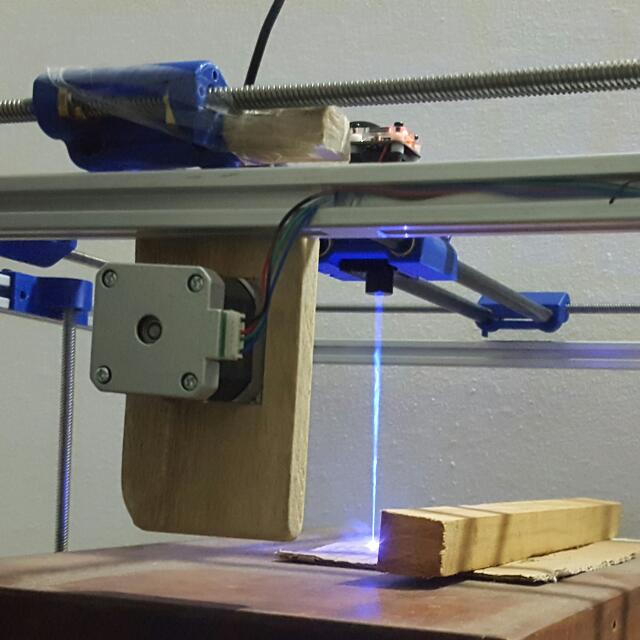
\includegraphics[width=0.35\textwidth]{./logo}~\\[1cm]

\textsc{\LARGE IFNTI - Sokodé}\\[1.5cm]

\textsc{\Large }\\[0.5cm]

% Title
\HRule \\[0.4cm]

{\huge \bfseries Imprimante 3D - Laser\\
Conception d'une imprimante 3D et d'une Graveuse Laser \\[0.4cm] }

\HRule \\[1.5cm]

% Author and supervisor
\begin{minipage}{0.4\textwidth}
\begin{flushleft} \large
\emph{Auteurs:}\\
\textsc{AYEVA Yaasiin}\\
\textsc{ISSA-TOURÉ Aziz}\\
\textsc{TCHASSONA TRAORÉ Walid}\\
\textsc{TÉOURI Samrou}\\
\textsc{TÉOURI Touré-Ydaou}
\end{flushleft}
\end{minipage}
\begin{minipage}{0.4\textwidth}
\begin{flushright} \large
\emph{Client:} \\
\textsc{IFNTI}\\
\emph{Référent:} \\
\textsc{Jean-Christophe CARRE}
\end{flushright}
\end{minipage}

\vfill

% Bottom of the page
{\large \today}

\end{center}
\end{titlepage}

%page blanche
\newpage
~
%ne pas numéroter cette page
\thispagestyle{empty}
\newpage

\renewcommand{\abstractnamefont}{\normalfont\Large\bfseries}
%\renewcommand{\abstracttextfont}{\normalfont\Huge}

\begin{abstract}
\hskip7mm

\begin{spacing}{1.3}

Janvier 2021 marque le début de la constitution des groupes pour les différents projets Arduino.  L'initiateur de cette idée est en effet l'instituteur Jean-Christophe CARRE dit "jc". Nos activités ont été réellement effectives à partir de Mars 2021. L'idée était d'être prêt pour les journées étudiantes qui avaient lieu le même mois. Notre groupe était organisé en cinq (5) membres sous la supervision de jc. Le squelette de l'imprimante 3D avait déjà été assemblé par jc. Le gros du travail résidait d'abord dans les branchements et les calculs liés au type de fonctionnement escompté de la machine. Il y avait aussi la configuration et le flashage de la firmware \textit{Marlin 2.0} (qui nous était totalement inconnue au début); Ceci pour permettre à la machine de fonctionner intelligemment et selon nos diverses attentes. Notre travail a porté également sur la conception 3D à partir du logiciel libre \textit{FreeCad} sous \textit{Linux}. Nous nous sommes également penché sur le dessin sur \textit{Inkscape} couplé avec la génération de \textit{g-code} pour les mouvements du Laser. Ce rapport rend compte de l'ensemble des activités menées sur ce projet. Il détaille aussi sur les branchements et configurations effectuées. Enfin il présente un guide pour aider à la manipulations de l'imprimante 3D.

\end{spacing}
\end{abstract}


\tableofcontents
\thispagestyle{empty}
\setcounter{page}{0}
%ne pas numéroter le sommaire

\newpage

%espacement entre les lignes d'un tableau
\renewcommand{\arraystretch}{1.5}

%====================== INCLUSION DES PARTIES ======================

~
\thispagestyle{empty}
%recommencer la numérotation des pages à "1"
\setcounter{page}{0}
\newpage

\part{Présentation du projet}

\section{Sujet}

Dans l'optique de créer des kits constructifs et des  outils  pour  activités  créatives  de  groupe, il apparaît indispensable de se munir soi-même d'une imprimante 3D et d'une graveuse laser ou découpeuse laser (conception en 2D). La première partie de notre sujet concerne la conception de la graveuse laser. (cf. fig. 1.1)%\\
%inclusion d'une mage dans le document
\begin{figure}[!h]
\begin{center}
%taille de l'image en largeur
%remplacer "width" par "height" pour régler la hauteur
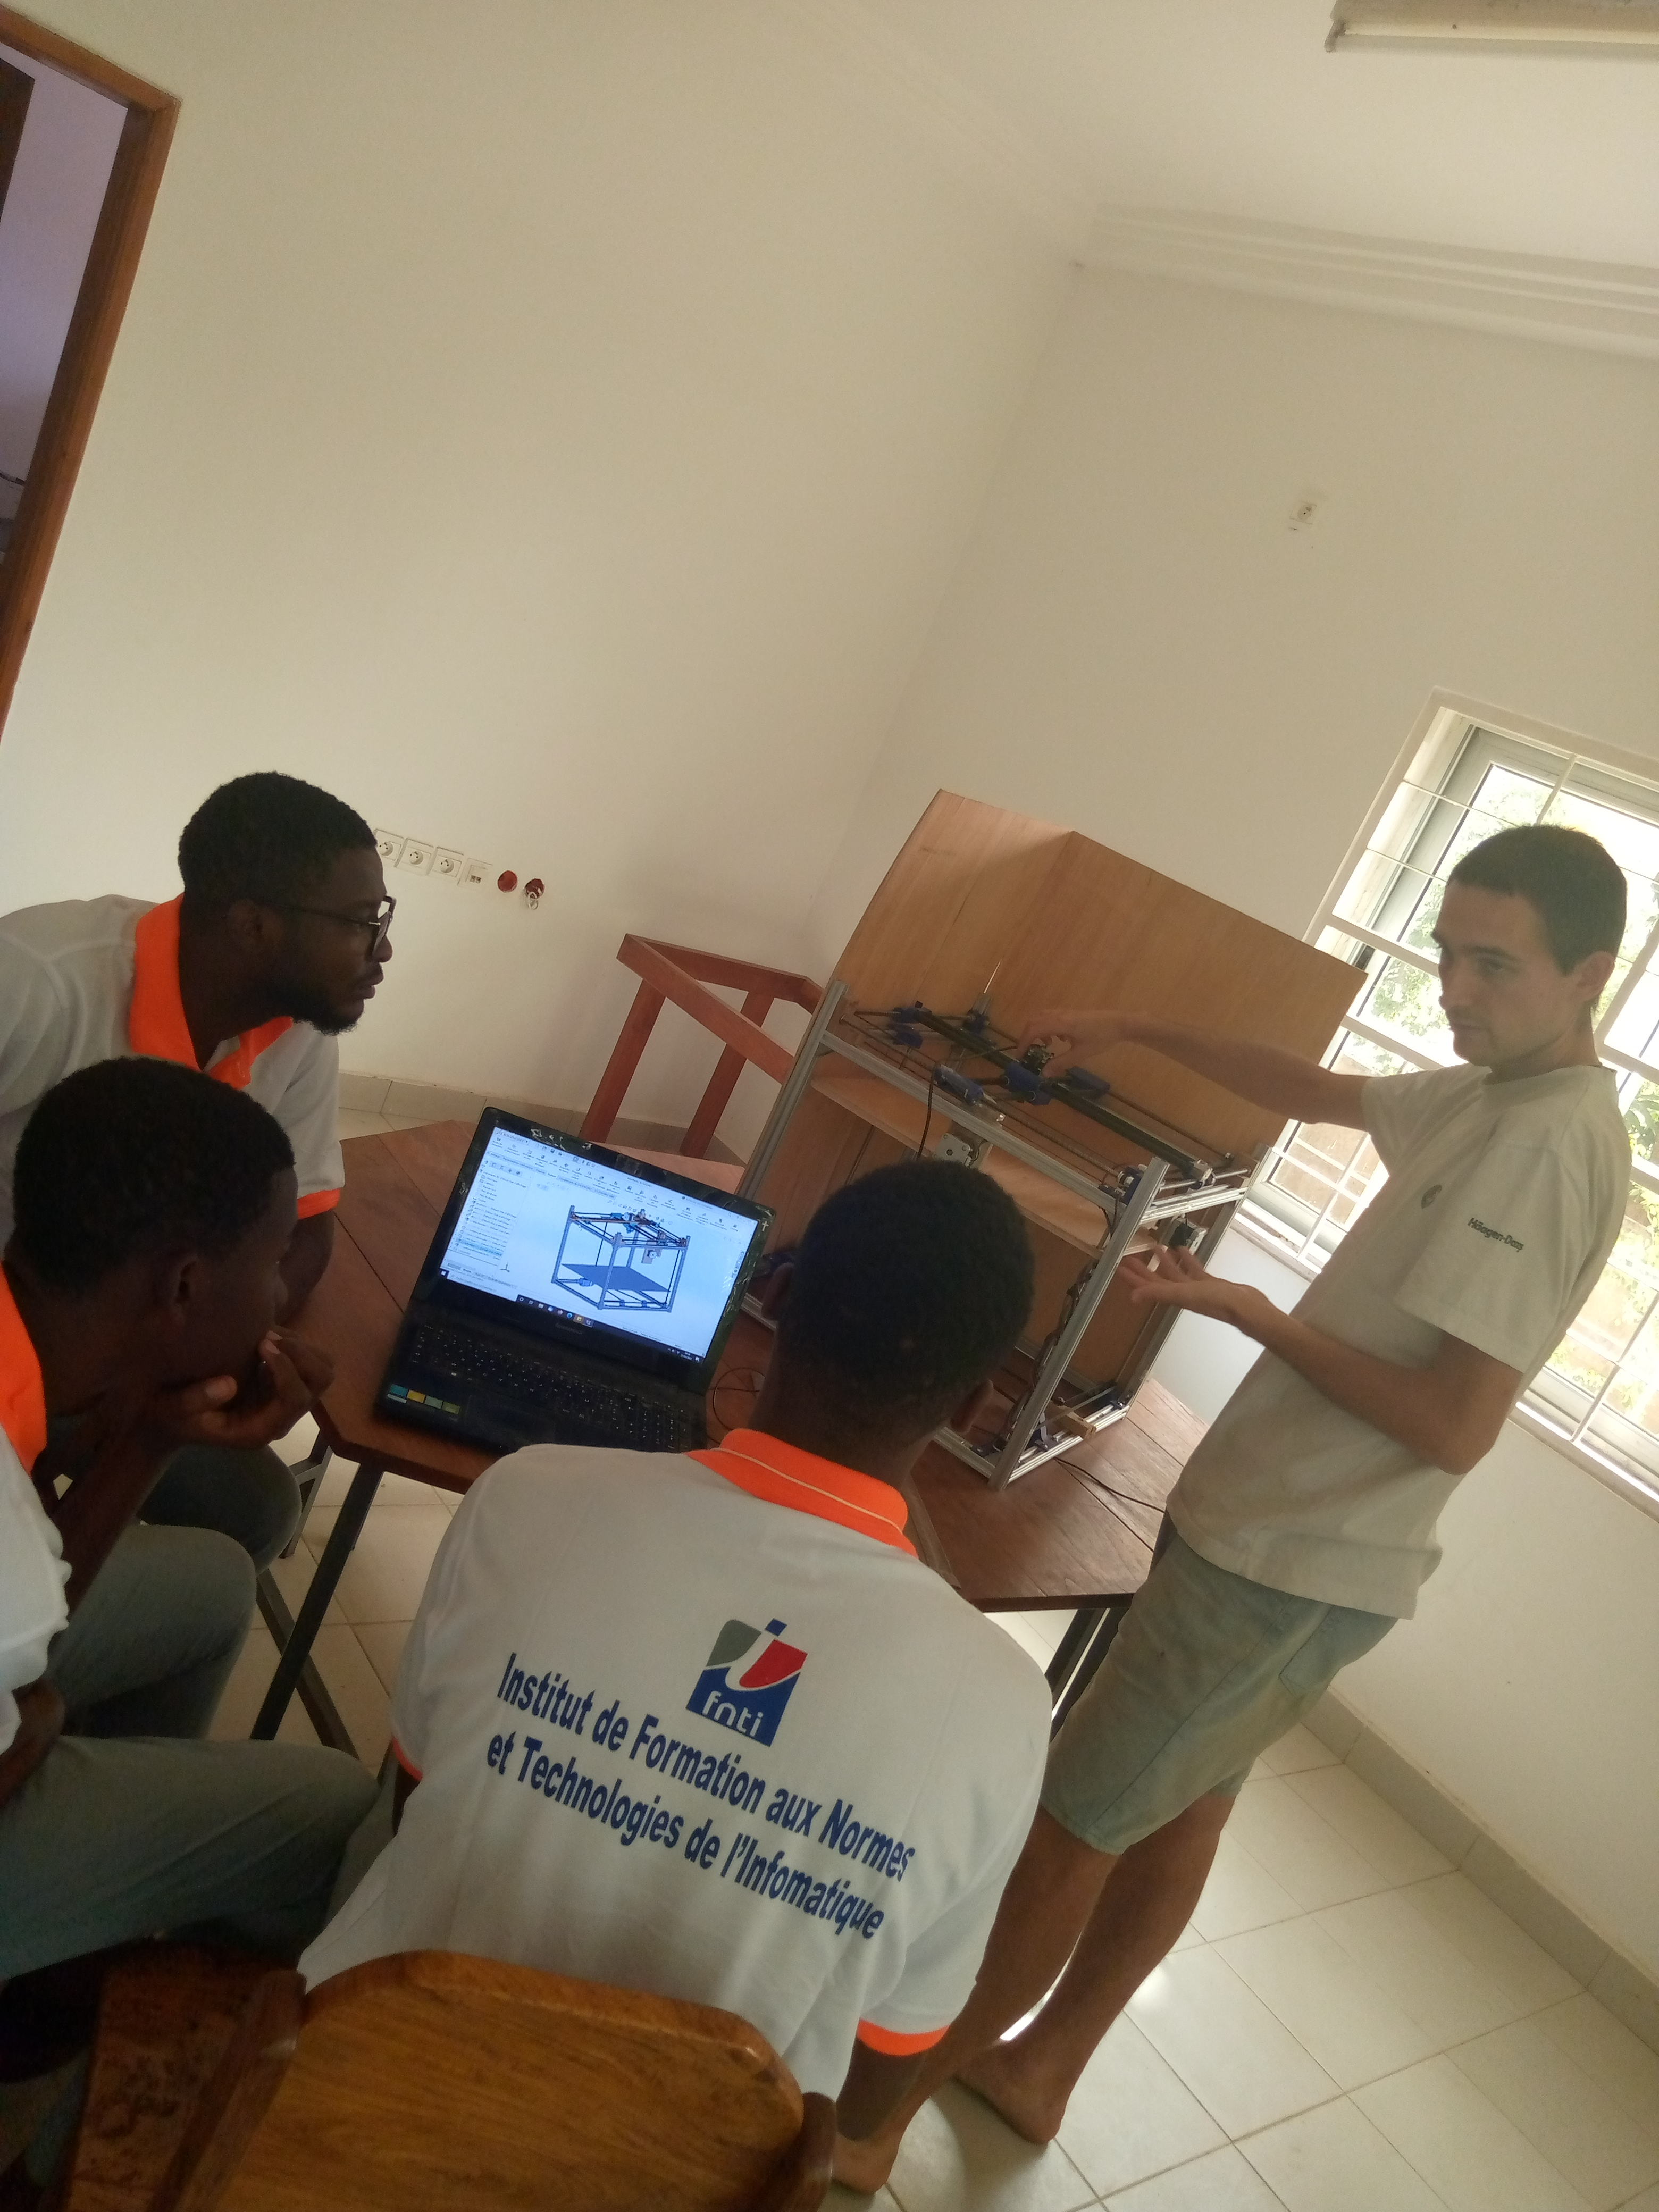
\includegraphics[width=13cm]{presentation/schema}
\end{center}
%légende de l'image
\caption{Squelette de l'imprimante 3D à la base}
\end{figure}\\

Selon Wikipédia, La découpe laser est un procédé de fabrication qui consiste à découper la matière grâce à une grande quantité d’énergie générée par un laser et concentrée sur une très faible surface. Cette découpe peut servir à faire un dessin, graver des caractères sur du bois par exemple. \\
%saut de paragraphe

La partie "graveuse laser" a été réalisée en deux semaines avec la collaboration de certains étudiants de première année. Le projet est cependant appelé à évoluer. La partie "imprimante 3D" viendra corroborer l'ensemble du projet.

\section{Problématique soulevée}
Le branchement et la mise en relation des composants matériels constituait un problème fondamental vu le temps qui nous était imparti. D'autre part il fallait s'occuper aussi du code qui fera fonctionner plus tard la machine. C'est à dire programmer les mouvements de la tête de laser, les commandes associées aux actions du laser ...

\section{Hypothèse de solution}

Il y avait ainsi deux grandes parties sur lesquelles il fallait se pencher. La partie mécanique et la partie code. Les étudiants de la première année s'occuperont exclusivement de cette partie sous notre supervision. Quant à nous qui avons accueilli le projet, La partie code nous sera consacrée. Et dans cette partie il fallait retenir en avance quelques points essentiels sur lesquels il fallait bosser.

\begin{itemize}
\item La configuration et le mode de fonctionnement escompté de la machine selon l'architecture dont nous disposons  (Core XY, Core YZ, ...) ;
\item Les déplacement horizontaux du laser selon les axes X et Y;
\item Les Commandes d'allumages, d'extinction du laser ...
\end{itemize}

La configuration de la firmware marlin 2.0\footnotemark était donc le gros du travail pour faire fonctionner l'imprimante.

\footnotetext{Marlin est un micrologiciel open source utilisé pour les imprimantes 3D et utilisant la plateforme Arduino.\\ \href{https://marlinfw.org/}{Consulter le site officiel de Marlin}}

\section{Analyse de l'existant}
Le squelette de l'imprimante 3D comportait déjà le minimum de matériel dont nous avions besoin. On avait entre autre :
\begin{itemize}
	\item La carte Arduino Mega
	\item La carte RAMPS v1.4 de RepRap
	\item La tête de laser
	\item Les moteurs pour les mouvements des axes X, Y et Z
	\item Un moniteur à molette avec un port SD
	\item deux capteurs de fin de course (sur les axes X et Y)
	\item Une source d'alimentation (power supply) qui transforme le 220V du secteur en 12V
\end{itemize}

\section{Besoins externes}
Sur le plan matériel, nous n'avions pas besoins de grand chose. Ce qui manquait était les compétences en code surtout; et de savoir quel composant branché à quel endroit. Il fallait donc passer du temps sur les sites officiels des constructeurs et dans divers forums en ligne pour en savoir plus. Nous avons donc mis à jour un dépôt Git dans lequel une section \textbf{documentation} rassemblait toutes nos trouvailles. Avant de débuter la configuration de la firmware, il était impératif pour nous de pouvoir répondre aux questions suivante :
\begin{itemize}
	\item Style escompté de l'imprimante : Cartesian, Delta, CoreXY, ou SCARA
    \item De quel type de driver board disposons nous : RAMPS, RUMBA, Teensy, etc.
    \item la carte Arduino compatible avec le driver board : Mega 2560
    \item Le nombre d'extrudeurs
    \item le stepping par millimètre pour les axes XYZ et les extrudeurs
    \item La position des capteurs de fin de course (Endstop)
	\item La marque et le modèle du contrôleur LCD dont nous disposons
    \item Modules complémentaires et composants personnalisés
\end{itemize}


 
%\chapter{Analyse des besoins}

Intro

\section{Besoins fonctionnels}

Après une analyse des besoins fonctionnels du projet, nous avons défini deux sous catégories. D'un côté, les besoins [...], de l'autre, les besoins [...].

\subsection{Sous-partie 1}

Bla

\subsection{Sous-partie 2}

Bla

\newpage

\section{Besoins non-fonctionnels}

Comme précédemment, nous avons choisi de distinguer deux catégories pour les besoins non-fonctionnels. D'une part, nous avons les besoins non-fonctionnels pour les [...], et d'autre part ceux pour [...]. Nous avons aussi pris en compte les contraintes de développement, que nous détaillerons à la fin de cette partie.

\subsection{Sous-partie 1}

Bla\\

Aperçu du rendu souhaité :

\begin{figure}[!h]
\begin{center}
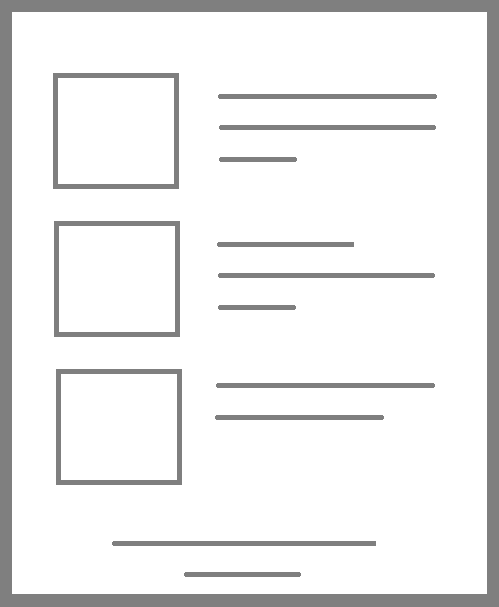
\includegraphics[height=10cm]{besoins/rendu}
\end{center}
\caption{Rendu attendu}
\end{figure}

\subsection{Sous-partie 2}

Bla

\newpage

\section{Développement}

Intro

\subsection{Tâches}

Bla\\


%tableau à taille fixée sur certaines colonnes (param sur la ligne \begin{tabularx}, voir wiki pour plus d'info sur la syntaxe
\begin{figure}[!h]
\begin{center}
\begin{tabularx}{17cm}{|c|p{6cm}|X|}
  \hline
  Priorité & Nom & Raison\\
  \hline
  1 & Tache 1 & Doit être vérifié en premier car sinon [...] \tabularnewline
  2 & Tache 2 & On doit pouvoir [...] \tabularnewline
  3 & Tache 3 & Comme les principales fonctionnalités permettant de tester sont opérationnelles, nous pouvons passer à cette tâche. \tabularnewline
  4 & Tache 4 & Parce que [...] \tabularnewline
  5 & Tache 5 & La tache 5 fait partie des principales [...]. \tabularnewline
  6 & Tache 6 & Dernière fonctionnalité essentielle à mettre en place. \tabularnewline
  7 & Tache 7 & Non-essentiel, mais apporterait un plus au projet. \tabularnewline
  8 & Tache 8 & Non-essentiel, mais apporterait un plus au projet. \tabularnewline
  \hline
\end{tabularx}
\end{center}
\caption{Tableau récapitulatif des tâches}
\end{figure}

\subsection{Tests}

Bla\\

\begin{figure}[!h]
\begin{center}
\begin{tabularx}{17cm}{|p{6cm}|X|}
  \hline
  Fonctionnalité & Test\\
  \hline
  Fonction 1 & Quand [...], vérifier [...]. \tabularnewline
  & Et quand [...], vérifier [...]. \tabularnewline
  Fonction 2 & Vérifier [...]. \tabularnewline
  Fonction 3 & Vérifier [...]. \tabularnewline
  Fonction 4 & Avoir [...]. \tabularnewline
  Fonction 5 & Accéder à [...]. \tabularnewline
   & Vérifier que [...]. \tabularnewline
  Fonction 6 & Accéder à [...]. \tabularnewline
   & Et vérifier [...]. \tabularnewline
  Fonction 7 & Installer [...]. \tabularnewline
   & Vérifier [...]. \tabularnewline
  Fonction 8 & Compter [...]. \tabularnewline
  \hline
\end{tabularx}
\end{center}
\caption{Tableau récapitulatif des tests}
\end{figure}

%\chapter{Autre partie}

Dans cette partie nous cherchons à décrire dans un premier temps [...], puis, c[...].

\section{Partie 1}

Intro

\subsection{Sous-partie 1}

\begin{figure}[!ht]
\begin{center}

\includegraphics[height=12cm]{autre_partie/image1}
\end{center}
\caption[autre partie générale]{autre partie image 1\protect\footnotemark}
%\floatfoot{Source: (Citation command)}
% avec le package "floatrow"
\end{figure}

%footnote protected pour apparaitre dans la légende d'une image
\footnotetext{Schéma d'après : \textit{Auteur 1 \& Propriétaire image}, LICENCE (cf. ref. \cite{cite4})}

\newpage{}

\subsection{Sous-partie 2}

\begin{figure}[!ht]
\begin{center}

\includegraphics[height=12cm]{autre_partie/image2}
\end{center}
\caption[autre partie]{autre partie globale de notre quelque chose}
\end{figure}

Nous retrouvons ici, blabla\footnote{Application bla - Interface blabla} [...].

\subsubsection{Sous-sous-partie 1}

Le bla (cf. ref. \cite{cite6}) est [...]:

\begin{itemize}
\item item1;
\item item2;
\item item3;
\item item4;
\item item5.
\end{itemize}

\newpage

\subsubsection{Sous-sous-partie 2}

%Les lignes :
% \setcounter{secnumdepth}{4}
% \setcounter{tocdepth}{4}
%dans le fichier "main.tex" permettent de faire en sorte que les paragraphes soient interprété comme des titres de niveau 5
\paragraph{Paragraphe 1 (agissant comme titre niveau 5)}
%forcer un saut de ligne
~\\
\hskip7mm

\begin{figure}[!ht]
\begin{center}

\includegraphics[height=6cm]{autre_partie/image3}
\end{center}
\caption[Structure d'unz autre chose]{Structure d'une autre chose\protect\footnotemark}
\end{figure}

Ce schéma représente bla.

\footnotetext{Schéma et explication d'après le wiki bla (cf. ref. \cite{cite0})}

\paragraph{Paragraphe 2}
~\\
\hskip7mm

%fixer les floats précédemment définis
%\FloatBarrier

Bla

\subparagraph{Sous-paragraphe 1}
~\\
\hskip7mm

Bla

\begin{figure}[H]
\begin{center}

\includegraphics[height=10cm]{autre_partie/image4}
\end{center}
\caption{Diagramme de truc}
\end{figure}

\subparagraph{Sous-paragraphe 2}
~\\
\hskip7mm

Bla\\

Bla

\subparagraph{Sous-paragraphe 3}
~\\
\hskip7mm

Bla

\subsubsection{Sous-sous-partie 3}

Bla

\section{Partie 2}

Bla

\footnotetext{D'après le schéma disponible sur la documentfation officielle disponible sur le site blalbla}

Bla

\subsection{Sous-partie 1}

Bla

\subsection{Sous-partie 2}

Bla

\paragraph*{Paragraphe 1 (n'apparaitra pas dans l'index)}
Bla

\paragraph*{Paragraphe 2}
Bla

\paragraph*{Paragraphe 3}
Bla

\subsection{Sous-partie 3}

Bla

\part{Travaux effectués et résultats}

\section{Partie 1 - Branchement et Mécanique}

Cette section n'est pas renseignée!
\section{Partie 2 - Code et configuration de la firmware}
À partir de la configuration par défaut, il faut dé-commenter le nécessaire et ajouter des paramètre fondamentales ou personnels. Toute section ou paramètre qui ne sera pas cité dans ce document est à sa valeur par défaut selon la configuration de marlin 2.0 .
Le code est subdivisé en plusieurs sections de paramètres.

\subsection{Hardware Info}
Il nous revenait dans cette section de : 
\begin{itemize}
	\item modifier la valeur du baudrate pour la fixer à 250000
	\item définir la motherboard convenable (BOARD\_RAMPS\_14\_EFF)
	\item désigner un nom pour l’imprimante (CUSTOM\_MACHINE\_NAME : rose)
\end{itemize}
Pour le deuxième tiret il revient à modifier le fichier \textbf{boards.h} pour choisir le paramétrage convenable.

\subsection{Extruder Info}
\begin{itemize}
	\item choix du nombre d'extrudeurs : 1
	\item diamètre de filament et nozzle\footnotemark (70 et singlenozzle)
\end{itemize}
\footnotetext{nozzle désigne la buse de l'extrudeur}

\subsection{Kinematics}
Le premier paramètre à configurer faisait référence à la cinématique de l'imprimante 3D. C'est à dire le style de mouvement de la tête de laser selon les axes XYZ. les instructions disaient de dé-commenter au moins une option de cinématique entre : COREXY, COREXZ, COREYZ, COREYX, COREZX, COREZY, MARKFORGED\_XY. Mais on se rend compte après que le style de mouvement de chacun de ces sept options ne correspond vraiment pas à nos attentes. Il se trouve qu'on peut laisser commenté toutes les options. Et il y aura un comportement par défaut qui correspondra au style de mouvement désiré. En effet, par défaut marlin fonctionnerait en cartésien (XYZ) (source \footnotemark)
\footnotetext{\href{https://www.lesimprimantes3d.fr/forum/topic/18036-probl\%C3\%A8me-pilotage-axe/?do=findComment&comment=230701}{Consulter le forum}}

\subsection{Endstops }
Dans cette rubrique qui concerne exclusivement les capteurs de fins de course (endstop), il fallait :
\begin{itemize}
	\item modifier la logique des endstops (true).
	\item fixer le stepper driver. Pour les pilotes non spécifiés, la valeur par défaut est A4988
	\item activer les pins (interrups) pour les capteurs de fin de course 
\end{itemize}

\subsection{Movement}
Cette section est propre aux paramètres de mouvements de l'imprimante.
\begin{itemize}
	\item spécification du microsteping de 1/4 considéré.
	\item spécification du rythme d'accélération pour ne pas faire souffrir la mécanique
\end{itemize}

\subsection{Drivers}
\begin{itemize}
	\item inversion du sens de rotation des moteurs selon les axes XYZ (false)
\end{itemize}

\subsection{Homing and Bounds}
\begin{itemize}
	\item modification de la taille du bed (X = 300, Y = 318)
\end{itemize}

\subsection{Additonal Features}
\begin{itemize}
	\item activation de l'estimation de temps d'impression : PRINTJOB\_TIMER\_AUTOSTART
\end{itemize}

\subsection{User Interface Language}
\begin{itemize}
	\item définition de la langue du moniteur LCD
	\item Activation du support de carte SD
	\item définition de la vitesse de transmission SPI (fixée à HALF\_SPEED)
\end{itemize}

\subsection{Encoder}
\begin{itemize}
	\item inversion du sens de la molette du moniteur
\end{itemize}

\subsection{LCD Controller}
\begin{itemize}
	\item configuration de l'écran (LCD controller with click-wheel.)
\end{itemize}

\newpage

\part{Bilan}

%Rappel du context
En définitive, au bout de deux semaines, nous avons réussi à mettre sur pied une découpeuse laser qui répond entièrement à nos attentes. Cependant quelques erreurs persistent.Il s'agit entre autre des mouvements selon l'axe Z (question de mécanique). Il y a aussi le homing qui n'est pas idéal. En ce sens que l'imprimante se plante un moment juste après un homing au démarrage. Ce qui peut fausser les repères suivies par la tête de laser. Mais nous n'en sommes visiblement qu'à la toute première version. Et le projet est appelé à évoluer. Cela nous permettra de corriger les différents bugs et d'avoir une version plus pratique et plus simple d'utilisation.

%%Ne pas numéroter cette partie
\part*{Annexes}
%Rajouter la ligne "Annexes" dans le sommaire
\addcontentsline{toc}{part}{Annexes}

\chapter*{Annexe 1}
\addcontentsline{toc}{chapter}{Annexe 1}

%changer le format des sections, subsections pour apparaittre sans le num de chapitre
\makeatletter
\renewcommand{\thesection}{\@arabic\c@section}
\makeatother

%recommencer la numérotation des section à "1"
\setcounter{section}{0}

Intro

\section{Partie 1}

Bla

\subsection{Sous-partie 1}

Bla

\subsection{Sous-partie 2}

Bla

\subsection{Sous-partie 3}

Bla

\section{Partie 2}

Bla

\subsection{Sous-partie 1}

Bla

\subsection{Sous-partie 2}

Bla

\subsection{Sous-partie 3}

Bla

\chapter*{Annexe 2}
\addcontentsline{toc}{chapter}{Annexe 2}

%recommencer la numérotation des section à "1"
\setcounter{section}{0}

Intro

\section*{Prérequis}
\addcontentsline{toc}{section}{Prérequis}

Bla

\begin{itemize}
\item item1;
\item item2;
\item item3;
\item item4.
\end{itemize}

Bla

\section{Partie 1}

Bla

\subsection{Sous-parie 1}

Bla

\subsection{Sous-parie 2}

Bla

\section{Partie 2}

\begin{center}
\textsc{Attention !}

\textit{Texte d'avertissement}
\end{center}

Bla

\newpage

\section{Partie 3}

Bla

\begin{figure}[!ht]
\begin{center}
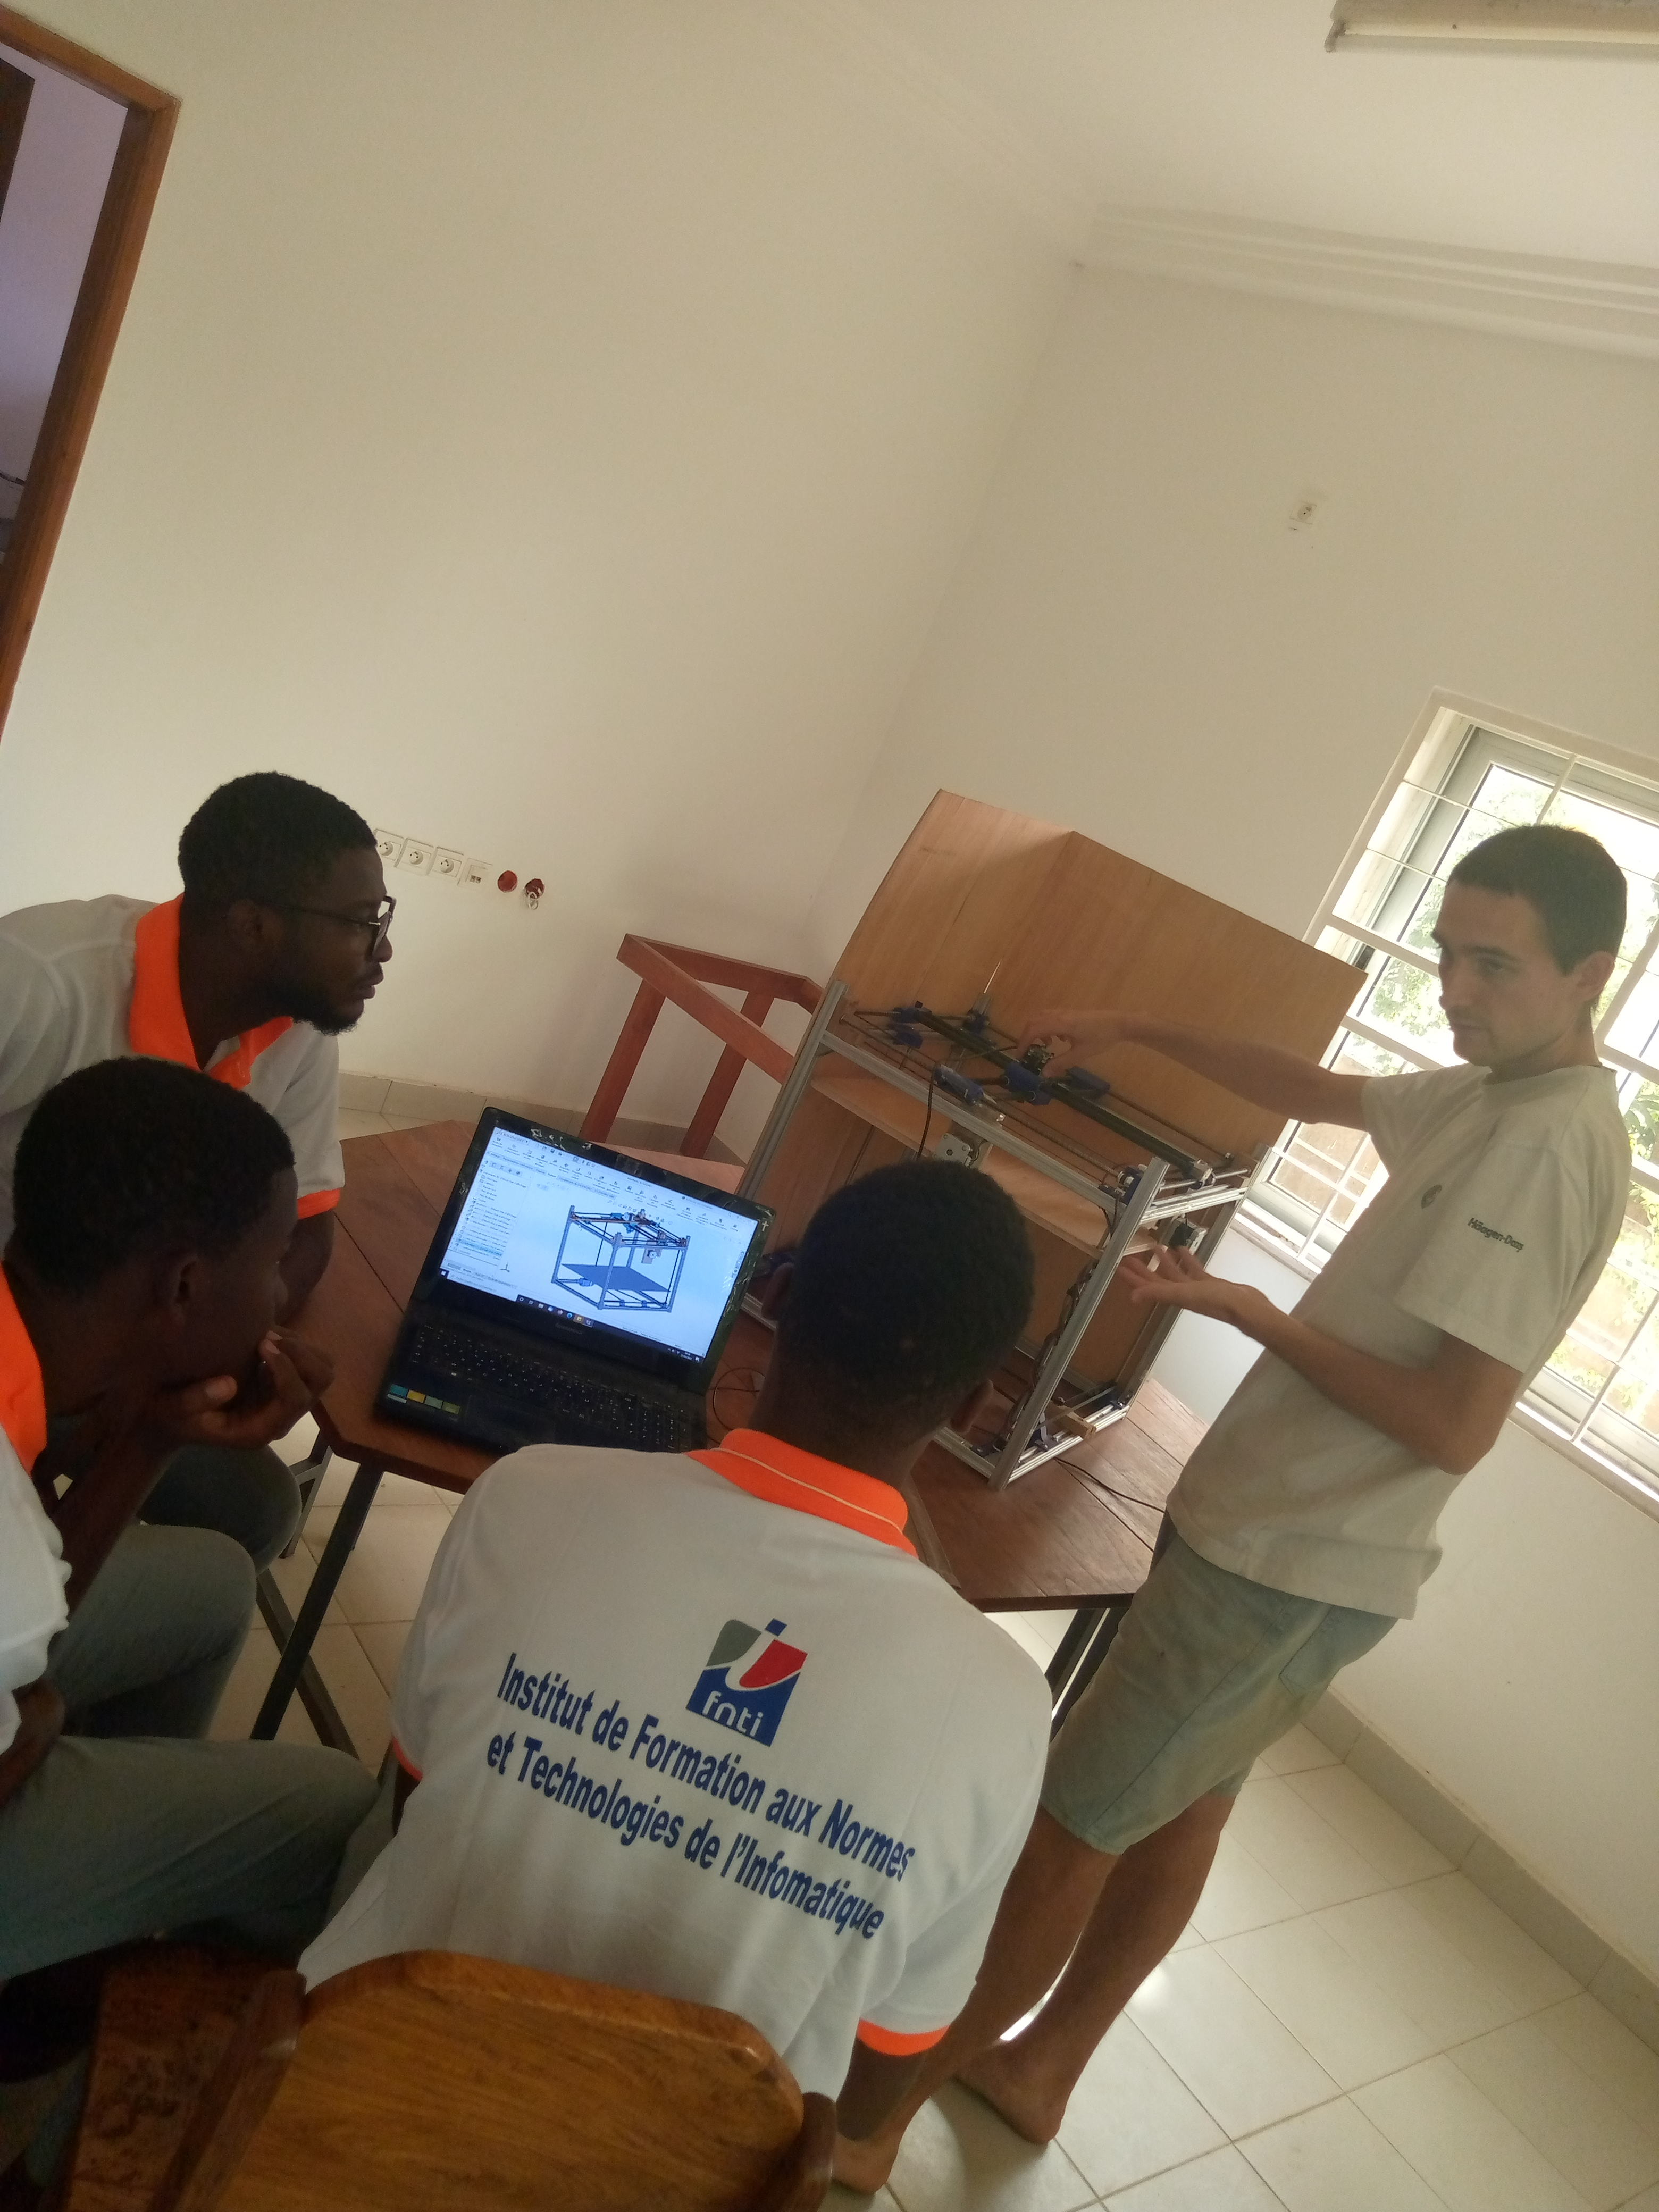
\includegraphics[height=8cm]{presentation/schema}
\end{center}
\caption[schema]{Presentation schema}
\end{figure}

\paragraph*{Paragraphe 1}
~\\
\hskip7mm

Bla

\paragraph*{Paragraphe 2}
~\\
\hskip7mm

Bla

\paragraph*{Paragraphe 3}
~\\
\hskip7mm

Bla

\newpage

%récupérer les citation avec "/footnotemark"
\nocite{*}

%choix du style de la biblio
\bibliographystyle{plain}
%inclusion de la biblio
\bibliography{bibliographie.bib}
%voir wiki pour plus d'information sur la syntaxe des entrées d'une bibliographie

\end{document}